\documentclass[tikz,border=6pt]{standalone}
\usepackage{lmodern}
\usepackage[T1]{fontenc}
\usepackage{amssymb}
\usetikzlibrary{arrows.meta,shapes.geometric,fit,backgrounds,calc,positioning}
\definecolor{letterA}{HTML}{1F5FA9}
\definecolor{letterB}{HTML}{B5651D}
\definecolor{order}{HTML}{8A9099}
\definecolor{boxline}{HTML}{B9BEC4}
\definecolor{boxfill}{HTML}{F4F5F7}
\definecolor{frozen}{HTML}{E9EEF6}
\definecolor{ref}{HTML}{A6ADB4}
\definecolor{hilite}{HTML}{DCE7F5}
\definecolor{ink}{HTML}{222629}
% Spot's LaTeX formula printer (`formula.to_str('latex')`) emits these.
\newcommand{\ttrue}{\top}
\newcommand{\ffalse}{\bot}
\newcommand{\limplies}{\rightarrow}
\newcommand{\liff}{\leftrightarrow}
\newcommand{\X}{\mathsf{X}\,}
\newcommand{\G}{\mathsf{G}\,}
\newcommand{\F}{\mathsf{F}\,}
\newcommand{\U}{\mathbin{\mathsf{U}}}
\newcommand{\W}{\mathbin{\mathsf{W}}}
\newcommand{\R}{\mathbin{\mathsf{R}}}
\newcommand{\M}{\mathbin{\mathsf{M}}}
\tikzset{
  % ---- classes and machines -------------------------------------
  cls/.style        = {circle, draw=ink, line width=.5pt, fill=white,
                       inner sep=0pt, minimum size=13mm, align=center,
                       font=\small},
  committed/.style  = {cls, double, double distance=1pt},
  entry/.style      = {draw=ink, line width=.8pt, -{Stealth[length=1.8mm]}},
  % ---- layers ----------------------------------------------------
  layerbox/.style   = {rounded corners=3pt, draw=boxline, fill=boxfill,
                       line width=.7pt},
  frozenbox/.style  = {layerbox, fill=frozen},
  layertag/.style   = {font=\scriptsize, text=ink, align=left,
                       inner sep=2pt},
  layername/.style  = {font=\scriptsize\bfseries, text=order},
  rorder/.style     = {draw=order, line width=2.2pt,
                       -{Stealth[length=3.2mm,width=3mm]}, opacity=.75},
  % ---- alphabet --------------------------------------------------
  ea/.style         = {draw=letterA, text=letterA, line width=.9pt,
                       -{Stealth[length=2mm]}},
  eb/.style         = {draw=letterB, text=letterB, line width=.9pt,
                       dashed, dash pattern=on 2.4pt off 1.6pt,
                       -{Stealth[length=2mm]}},
  eall/.style       = {draw=ink, text=ink, line width=.9pt,
                       -{Stealth[length=2mm]}},
  elab/.style       = {font=\scriptsize, inner sep=1.5pt,
                       fill=white, fill opacity=.85, text opacity=1},
  % ---- formula panels --------------------------------------------
  opnode/.style     = {rounded corners=2pt, draw=ink, fill=white,
                       line width=.5pt, inner sep=3pt, minimum height=5.5mm,
                       minimum width=9mm, font=\small, align=center},
  ophandle/.style   = {opnode, draw=order, fill=boxfill,
                       font=\footnotesize},
  opatom/.style     = {opnode, draw=letterA, text=letterA,
                       font=\small\ttfamily},
  dagedge/.style    = {draw=ink, line width=.6pt, -{Stealth[length=1.6mm]}},
  refedge/.style    = {draw=ref, line width=.5pt, densely dotted,
                       -{Stealth[length=1.4mm]}},
  slot/.style       = {font=\tiny, text=ref, inner sep=1pt, fill=white,
                       fill opacity=.85, text opacity=1},
  badge/.style      = {font=\tiny, text=order, inner sep=1pt},
  elide/.style      = {font=\scriptsize\itshape, text=order, align=center},
  panelcap/.style   = {font=\scriptsize, text=ink, align=center},
  % ---- derivation panels ------------------------------------------
  minicls/.style    = {circle, draw=order, fill=white, line width=.3pt,
                       inner sep=0pt, minimum size=3.4mm, font=\tiny,
                       text=ink},
  minibox/.style    = {rounded corners=1.4pt, draw=boxline, fill=white,
                       line width=.4pt},
  minidone/.style   = {minibox, fill=boxfill},
  minilive/.style   = {minibox, draw=letterA, fill=hilite, line width=.7pt},
  miniorder/.style  = {draw=order, line width=.9pt,
                       -{Stealth[length=1.5mm]}, opacity=.6},
  blockhead/.style  = {font=\small\bfseries, text=ink, anchor=west},
  blocknote/.style  = {font=\scriptsize\itshape, text=order, anchor=west},
  brick/.style      = {font=\small, text=ink, anchor=west},
  rulelab/.style    = {font=\scriptsize\itshape, text=order, anchor=west},
}

\begin{document}
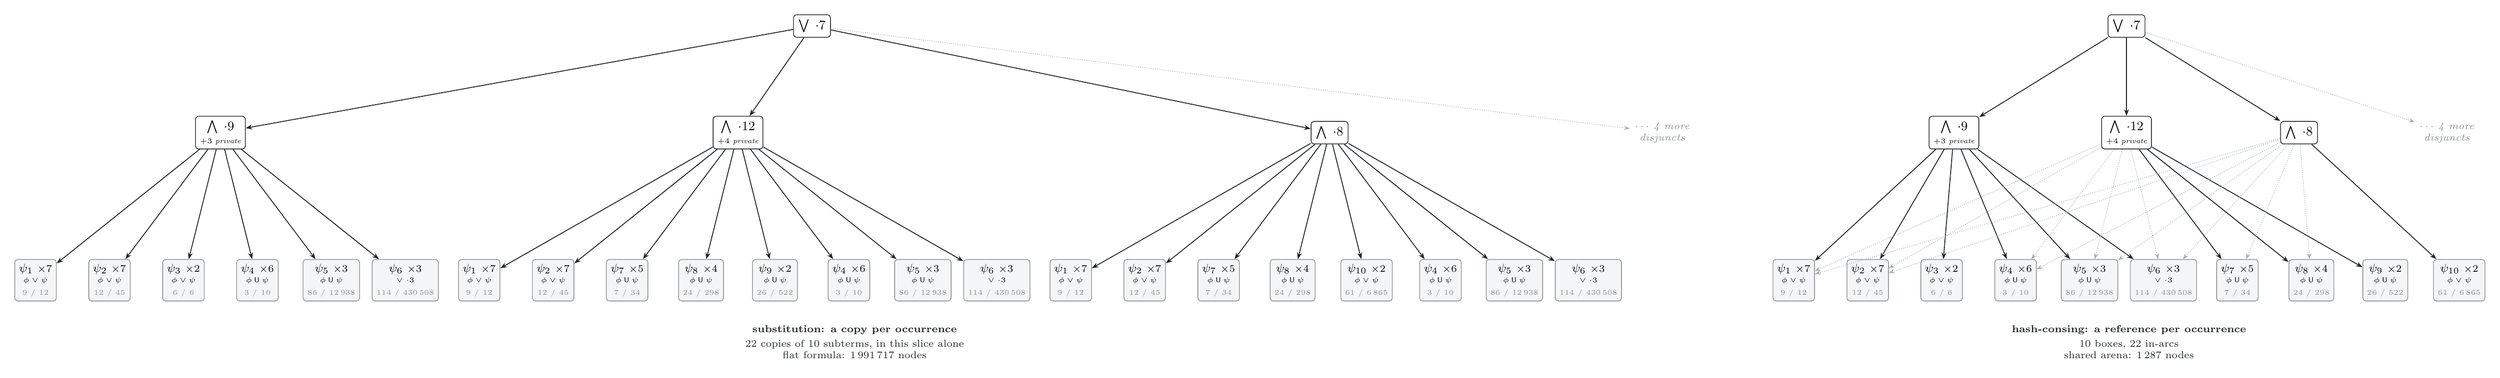
\begin{tikzpicture}
\begin{scope}[local bounding box=treepanel]
  \node[opnode] (troot) at (0,0) {$\bigvee\;{\cdot}7$};
  \node[opnode] (tp1167) at (-14.40,-2.6) {$\bigwedge\;{\cdot}9$\\[-2pt]{\tiny\itshape $+3$ private}};
  \draw[dagedge] (troot) --  (tp1167);
  \node[ophandle] (t1167h424) at (-18.90,-6.2) {$\psi_{1}$ {\scriptsize$\times$7}\\[-2pt]{\tiny $\phi \lor \psi$}\\[-1pt]{\tiny\textcolor{order}{9 / 12}}};
  \draw[dagedge] (tp1167) --  (t1167h424);
  \node[ophandle] (t1167h989) at (-17.10,-6.2) {$\psi_{2}$ {\scriptsize$\times$7}\\[-2pt]{\tiny $\phi \lor \psi$}\\[-1pt]{\tiny\textcolor{order}{12 / 45}}};
  \draw[dagedge] (tp1167) --  (t1167h989);
  \node[ophandle] (t1167h429) at (-15.30,-6.2) {$\psi_{3}$ {\scriptsize$\times$2}\\[-2pt]{\tiny $\phi \lor \psi$}\\[-1pt]{\tiny\textcolor{order}{6 / 6}}};
  \draw[dagedge] (tp1167) --  (t1167h429);
  \node[ophandle] (t1167h1075) at (-13.50,-6.2) {$\psi_{4}$ {\scriptsize$\times$6}\\[-2pt]{\tiny $\phi \U \psi$}\\[-1pt]{\tiny\textcolor{order}{3 / 10}}};
  \draw[dagedge] (tp1167) --  (t1167h1075);
  \node[ophandle] (t1167h1102) at (-11.70,-6.2) {$\psi_{5}$ {\scriptsize$\times$3}\\[-2pt]{\tiny $\phi \U \psi$}\\[-1pt]{\tiny\textcolor{order}{86 / 12\,938}}};
  \draw[dagedge] (tp1167) --  (t1167h1102);
  \node[ophandle] (t1167h1164) at (-9.90,-6.2) {$\psi_{6}$ {\scriptsize$\times$3}\\[-2pt]{\tiny $\lor\;{\cdot}3$}\\[-1pt]{\tiny\textcolor{order}{114 / 430\,508}}};
  \draw[dagedge] (tp1167) --  (t1167h1164);
  \node[opnode] (tp1196) at (-1.80,-2.6) {$\bigwedge\;{\cdot}12$\\[-2pt]{\tiny\itshape $+4$ private}};
  \draw[dagedge] (troot) --  (tp1196);
  \node[ophandle] (t1196h424) at (-8.10,-6.2) {$\psi_{1}$ {\scriptsize$\times$7}\\[-2pt]{\tiny $\phi \lor \psi$}\\[-1pt]{\tiny\textcolor{order}{9 / 12}}};
  \draw[dagedge] (tp1196) --  (t1196h424);
  \node[ophandle] (t1196h989) at (-6.30,-6.2) {$\psi_{2}$ {\scriptsize$\times$7}\\[-2pt]{\tiny $\phi \lor \psi$}\\[-1pt]{\tiny\textcolor{order}{12 / 45}}};
  \draw[dagedge] (tp1196) --  (t1196h989);
  \node[ophandle] (t1196h997) at (-4.50,-6.2) {$\psi_{7}$ {\scriptsize$\times$5}\\[-2pt]{\tiny $\phi \U \psi$}\\[-1pt]{\tiny\textcolor{order}{7 / 34}}};
  \draw[dagedge] (tp1196) --  (t1196h997);
  \node[ophandle] (t1196h1172) at (-2.70,-6.2) {$\psi_{8}$ {\scriptsize$\times$4}\\[-2pt]{\tiny $\phi \U \psi$}\\[-1pt]{\tiny\textcolor{order}{24 / 298}}};
  \draw[dagedge] (tp1196) --  (t1196h1172);
  \node[ophandle] (t1196h1034) at (-0.90,-6.2) {$\psi_{9}$ {\scriptsize$\times$2}\\[-2pt]{\tiny $\phi \U \psi$}\\[-1pt]{\tiny\textcolor{order}{26 / 522}}};
  \draw[dagedge] (tp1196) --  (t1196h1034);
  \node[ophandle] (t1196h1075) at (0.90,-6.2) {$\psi_{4}$ {\scriptsize$\times$6}\\[-2pt]{\tiny $\phi \U \psi$}\\[-1pt]{\tiny\textcolor{order}{3 / 10}}};
  \draw[dagedge] (tp1196) --  (t1196h1075);
  \node[ophandle] (t1196h1102) at (2.70,-6.2) {$\psi_{5}$ {\scriptsize$\times$3}\\[-2pt]{\tiny $\phi \U \psi$}\\[-1pt]{\tiny\textcolor{order}{86 / 12\,938}}};
  \draw[dagedge] (tp1196) --  (t1196h1102);
  \node[ophandle] (t1196h1164) at (4.50,-6.2) {$\psi_{6}$ {\scriptsize$\times$3}\\[-2pt]{\tiny $\lor\;{\cdot}3$}\\[-1pt]{\tiny\textcolor{order}{114 / 430\,508}}};
  \draw[dagedge] (tp1196) --  (t1196h1164);
  \node[opnode] (tp1230) at (12.60,-2.6) {$\bigwedge\;{\cdot}8$};
  \draw[dagedge] (troot) --  (tp1230);
  \node[ophandle] (t1230h424) at (6.30,-6.2) {$\psi_{1}$ {\scriptsize$\times$7}\\[-2pt]{\tiny $\phi \lor \psi$}\\[-1pt]{\tiny\textcolor{order}{9 / 12}}};
  \draw[dagedge] (tp1230) --  (t1230h424);
  \node[ophandle] (t1230h989) at (8.10,-6.2) {$\psi_{2}$ {\scriptsize$\times$7}\\[-2pt]{\tiny $\phi \lor \psi$}\\[-1pt]{\tiny\textcolor{order}{12 / 45}}};
  \draw[dagedge] (tp1230) --  (t1230h989);
  \node[ophandle] (t1230h997) at (9.90,-6.2) {$\psi_{7}$ {\scriptsize$\times$5}\\[-2pt]{\tiny $\phi \U \psi$}\\[-1pt]{\tiny\textcolor{order}{7 / 34}}};
  \draw[dagedge] (tp1230) --  (t1230h997);
  \node[ophandle] (t1230h1172) at (11.70,-6.2) {$\psi_{8}$ {\scriptsize$\times$4}\\[-2pt]{\tiny $\phi \U \psi$}\\[-1pt]{\tiny\textcolor{order}{24 / 298}}};
  \draw[dagedge] (tp1230) --  (t1230h1172);
  \node[ophandle] (t1230h1218) at (13.50,-6.2) {$\psi_{10}$ {\scriptsize$\times$2}\\[-2pt]{\tiny $\phi \lor \psi$}\\[-1pt]{\tiny\textcolor{order}{61 / 6\,865}}};
  \draw[dagedge] (tp1230) --  (t1230h1218);
  \node[ophandle] (t1230h1075) at (15.30,-6.2) {$\psi_{4}$ {\scriptsize$\times$6}\\[-2pt]{\tiny $\phi \U \psi$}\\[-1pt]{\tiny\textcolor{order}{3 / 10}}};
  \draw[dagedge] (tp1230) --  (t1230h1075);
  \node[ophandle] (t1230h1102) at (17.10,-6.2) {$\psi_{5}$ {\scriptsize$\times$3}\\[-2pt]{\tiny $\phi \U \psi$}\\[-1pt]{\tiny\textcolor{order}{86 / 12\,938}}};
  \draw[dagedge] (tp1230) --  (t1230h1102);
  \node[ophandle] (t1230h1164) at (18.90,-6.2) {$\psi_{6}$ {\scriptsize$\times$3}\\[-2pt]{\tiny $\lor\;{\cdot}3$}\\[-1pt]{\tiny\textcolor{order}{114 / 430\,508}}};
  \draw[dagedge] (tp1230) --  (t1230h1164);
  \node[elide] (telide) at (20.70,-2.6) {$\cdots$ 4 more\\disjuncts};
  \draw[refedge] (troot) -- (telide);
\end{scope}
\begin{scope}[xshift=32cm]
\begin{scope}[local bounding box=dagpanel]
  \node[opnode] (droot) at (0,0) {$\bigvee\;{\cdot}7$};
  \node[opnode] (dp1167) at (-4.20,-2.6) {$\bigwedge\;{\cdot}9$\\[-2pt]{\tiny\itshape $+3$ private}};
  \draw[dagedge] (droot) --  (dp1167);
  \node[opnode] (dp1196) at (0.00,-2.6) {$\bigwedge\;{\cdot}12$\\[-2pt]{\tiny\itshape $+4$ private}};
  \draw[dagedge] (droot) --  (dp1196);
  \node[opnode] (dp1230) at (4.20,-2.6) {$\bigwedge\;{\cdot}8$};
  \draw[dagedge] (droot) --  (dp1230);
  \node[elide] (delide) at (7.8,-2.6) {$\cdots$ 4 more\\disjuncts};
  \draw[refedge] (droot) -- (delide);
  \node[ophandle] (dh424) at (-8.10,-6.2) {$\psi_{1}$ {\scriptsize$\times$7}\\[-2pt]{\tiny $\phi \lor \psi$}\\[-1pt]{\tiny\textcolor{order}{9 / 12}}};
  \node[ophandle] (dh989) at (-6.30,-6.2) {$\psi_{2}$ {\scriptsize$\times$7}\\[-2pt]{\tiny $\phi \lor \psi$}\\[-1pt]{\tiny\textcolor{order}{12 / 45}}};
  \node[ophandle] (dh429) at (-4.50,-6.2) {$\psi_{3}$ {\scriptsize$\times$2}\\[-2pt]{\tiny $\phi \lor \psi$}\\[-1pt]{\tiny\textcolor{order}{6 / 6}}};
  \node[ophandle] (dh1075) at (-2.70,-6.2) {$\psi_{4}$ {\scriptsize$\times$6}\\[-2pt]{\tiny $\phi \U \psi$}\\[-1pt]{\tiny\textcolor{order}{3 / 10}}};
  \node[ophandle] (dh1102) at (-0.90,-6.2) {$\psi_{5}$ {\scriptsize$\times$3}\\[-2pt]{\tiny $\phi \U \psi$}\\[-1pt]{\tiny\textcolor{order}{86 / 12\,938}}};
  \node[ophandle] (dh1164) at (0.90,-6.2) {$\psi_{6}$ {\scriptsize$\times$3}\\[-2pt]{\tiny $\lor\;{\cdot}3$}\\[-1pt]{\tiny\textcolor{order}{114 / 430\,508}}};
  \node[ophandle] (dh997) at (2.70,-6.2) {$\psi_{7}$ {\scriptsize$\times$5}\\[-2pt]{\tiny $\phi \U \psi$}\\[-1pt]{\tiny\textcolor{order}{7 / 34}}};
  \node[ophandle] (dh1172) at (4.50,-6.2) {$\psi_{8}$ {\scriptsize$\times$4}\\[-2pt]{\tiny $\phi \U \psi$}\\[-1pt]{\tiny\textcolor{order}{24 / 298}}};
  \node[ophandle] (dh1034) at (6.30,-6.2) {$\psi_{9}$ {\scriptsize$\times$2}\\[-2pt]{\tiny $\phi \U \psi$}\\[-1pt]{\tiny\textcolor{order}{26 / 522}}};
  \node[ophandle] (dh1218) at (8.10,-6.2) {$\psi_{10}$ {\scriptsize$\times$2}\\[-2pt]{\tiny $\phi \lor \psi$}\\[-1pt]{\tiny\textcolor{order}{61 / 6\,865}}};
  \draw[dagedge] (dp1167) --  (dh424);
  \draw[dagedge] (dp1167) --  (dh989);
  \draw[dagedge] (dp1167) --  (dh429);
  \draw[dagedge] (dp1167) --  (dh1075);
  \draw[dagedge] (dp1167) --  (dh1102);
  \draw[dagedge] (dp1167) --  (dh1164);
  \draw[refedge] (dp1196) --  (dh424);
  \draw[refedge] (dp1196) --  (dh989);
  \draw[dagedge] (dp1196) --  (dh997);
  \draw[dagedge] (dp1196) --  (dh1172);
  \draw[dagedge] (dp1196) --  (dh1034);
  \draw[refedge] (dp1196) --  (dh1075);
  \draw[refedge] (dp1196) --  (dh1102);
  \draw[refedge] (dp1196) --  (dh1164);
  \draw[refedge] (dp1230) --  (dh424);
  \draw[refedge] (dp1230) --  (dh989);
  \draw[refedge] (dp1230) --  (dh997);
  \draw[refedge] (dp1230) --  (dh1172);
  \draw[dagedge] (dp1230) --  (dh1218);
  \draw[refedge] (dp1230) --  (dh1075);
  \draw[refedge] (dp1230) --  (dh1102);
  \draw[refedge] (dp1230) --  (dh1164);
\end{scope}
\end{scope}
\node[panelcap] at ($(treepanel.south)+(0,-1.0)$) {\textbf{substitution: a copy per occurrence}\\[2pt]22 copies of 10 subterms, in this slice alone\\flat formula: 1\,991\,717 nodes};
\node[panelcap] at ($(dagpanel.south)+(0,-1.0)$) {\textbf{hash-consing: a reference per occurrence}\\[2pt]10 boxes, 22 in-arcs\\shared arena: 1\,287 nodes};
\end{tikzpicture}
\end{document}
